% =====================================================================
%  Fig. 1 (clean redraw) -- end-to-end pipeline of the study, standalone TikZ.
%
%  Build : tectonic fig_pipeline_clean.tex   (XeTeX; page = 17.8 cm wide x 8.98 cm high)
%  Style : MLOps-architecture look (Kreuzberger et al.): light-grey stage panels with a
%          blue letter tag, white boxes with thin dark borders, one thin strip of secondary
%          text per panel, dashed grey zone separators, one legend row.
%  Colours (only these): panel E7E7E7, strip F4F4F4, box white / 404040 (0.5 pt), accent blue 4472C4,
%          "ours" fill DCE6F5 / blue 0.9 pt, text 222222, separators + zone names A6A6A6, arrows 404040.
%  Type  : Helvetica; panel titles bold 8 bp, box text 7.5 bp, strips/legend/labels 7 bp (nothing below
%          7 bp).  Sizes are given in TeX pt = bp x 1.00375 (8.03 / 7.53 / 7.03).
%  Layout: top zone = panels A, B; bottom zone = panels C, D (all coordinates in cm, origin bottom-left;
%          the bounding box is fixed by \useasboundingbox so the page is exactly 17.8 cm wide).
%  Flow  : A -> B along the top; one return line from B4 to the input column of C; C -> D below.
%          Solid arrows = data flow, dashed arrows = label flow, dotted lines = time reference.
%  Panel B (v12): time is drawn as an axis between the two data boxes, never as boxes joined by arrows.
%          Raw telemetry splits into the inputs (records before the cut, above the axis) and the labels
%          (kill events in the label window, below the axis); dotted lines tie each box to its window.
%  Labels (2026-10-08): every term matches the section that defines it (cutoff, habitat context with its four
%          constructs, our design, adapted designs); panels A-D follow Secs. III-A to III-D.
%  Panel C (v12): each input set points only at the design that uses it (habitat block -> RQ1 model and,
%          with the other team features, our design; Sagong and KRAFTON inputs -> adapted designs);
%          the stepwise decomposition hangs from a bracket under the RQ2 pair it decomposes.
%  v16 (2026-10-08): our design lists the regularized logistic baseline; RQ3 adds equal-trial tuning with the
%          exploratory GATv2 graph model; the strip adds graph controls; Metrics add calibration slope and top-3
%          capture.  The bottom zone grows 0.46 cm downward; the top zone keeps its coordinates.  The habitat box
%          names movement residual, as Sec. 4.1 defines it.
%          Page budget: zone names and separators removed, the top zone lowered 0.22 cm and the legend raised
%          0.23 cm (height 9.43 -> 8.98 cm).
%  External review (2026-10-09): panel D separates 11-cohort synthesis from 2-cohort controls and names the
%          match-phase centering diagnostic and the clustered SEs of RQ1; RQ3 names the horizon; panel B shows observed
%          alive status, the retrospective risk set, and the symbols a_{m,k}, b_{m,k}, b_{m,k+1}.
%          A symbol key under the legend explains m, i, k, a_{m,k}, b_{m,k}, b_{m,k+1}, T_{m,i}, and Y.
%  v17 (2026-10-09, evaluation-unit framing): RQ1 = matched objective controls (top box, replaces the ecological
%          hazard model, which moved to the supplementary notes), RQ2 = adapted vs our designs, RQ3 = inputs and
%          structure.  The top box feeds the predicted-risk store like the other analyses; Metrics stress the
%          within-match AUC and the match-phase centering diagnostic.
%  v18 (2026-10-09, evaluation-paper frame): two RQs (RQ1 objective controls, RQ2 design comparisons with the design
%          contrasts under the bracket); no 'ours' styling or legend entry; 'Reference designs' replaces 'Our design';
%          the input box names habitat and team features; the objective box adds the offset-only control.
%  v17b (2026-10-09, no appendix): the strips of panels C and D are removed, the bottom zone ends at 0.58, the legend
%          moves up 0.42 cm, and the symbol key is one line (Y is defined in the label box); height 9.64 -> 8.82 cm.
% =====================================================================
\documentclass[tikz,border=2pt]{standalone}
\usepackage{fix-cm}
\usepackage[T1]{fontenc}
\usepackage[scaled=1]{helvet}
\renewcommand\familydefault\sfdefault
\usepackage{fontawesome5}
\usetikzlibrary{arrows.meta}
% ---- type sizes (TeX pt; 8.03 pt = 8 bp, 7.53 pt = 7.5 bp, 7.03 pt = 7 bp) ----
\newcommand{\fTitle}{\fontsize{8.03}{9.4}\selectfont\bfseries}   % panel titles
\newcommand{\fLetter}{\fontsize{8.03}{9.4}\selectfont\bfseries}  % panel tag letter
\newcommand{\fBox}{\fontsize{7.53}{8.6}\selectfont}              % box text
\newcommand{\fZone}{\fontsize{7.53}{8.6}\selectfont\bfseries}    % zone names
\newcommand{\fSmall}{\fontsize{7.03}{8.2}\selectfont}            % strips, legend, edge labels
\newcommand{\fRQ}{\fontsize{7.03}{8.2}\selectfont\bfseries}      % RQ tags
\newcommand{\fSmallI}{\fontsize{7.03}{8.2}\selectfont\itshape}      % strips and arrow labels (italic)
\DeclareMathSizes{8.03}{8.03}{7.03}{7.03}
\DeclareMathSizes{7.53}{8.03}{7.03}{7.03}
\DeclareMathSizes{7.03}{8.03}{7.03}{7.03}
% ---- palette ----
\definecolor{panelF}{HTML}{E7E7E7}\definecolor{stripF}{HTML}{F4F4F4}
\definecolor{blueC}{HTML}{4472C4}\definecolor{oursF}{HTML}{DCE6F5}
\definecolor{txtC}{HTML}{222222}\definecolor{zoneC}{HTML}{A6A6A6}
\definecolor{ink}{HTML}{404040}
\definecolor{detC}{HTML}{555555}\definecolor{greyT}{HTML}{595959}\definecolor{greyD}{HTML}{7F7F7F}  % detail lines, strips/labels/adapted titles, adapted details
\definecolor{oursT}{HTML}{2F5597}\definecolor{verC}{HTML}{D55E00}                                      % emphasis: dark blue, vermilion
\newcommand{\md}{\ \textperiodcentered\ }
\newcommand{\bT}[2]{{\bfseries\color{#1}#2}}                                       % box title: bold, 7.5 bp (node font), colour #1
\newcommand{\bD}[2]{{\fontsize{7.03}{8.2}\selectfont\color{#1}#2}}                 % box detail line: regular 7 bp, colour #1
\newcommand{\cylry}{0.062}
\tikzset{
  >=Stealth,
  every node/.style={text=txtC, inner sep=0pt, outer sep=0pt, font=\fBox},
  panel/.style={fill=panelF, draw=none, rounded corners=2.5pt},
  box/.style={draw=ink, fill=white, line width=0.5pt},
  ours/.style={draw=blueC, fill=oursF, line width=0.9pt},
  edge/.style={draw=ink, line width=0.6pt, -{Stealth[length=3.6pt,width=3.0pt]}},
  dedge/.style={edge, dash pattern=on 2.2pt off 1.6pt},
  lineplain/.style={draw=ink, line width=0.6pt},
  dlineplain/.style={draw=ink, line width=0.6pt, dash pattern=on 2.2pt off 1.6pt},
  tref/.style={draw=ink, line width=0.55pt, dash pattern=on 0.55pt off 1.25pt},
  sep/.style={draw=zoneC, line width=0.5pt, dash pattern=on 3pt off 2.2pt},
  axis/.style={draw=ink, line width=0.5pt, -{Stealth[length=3.6pt,width=3.0pt]}},
  tick/.style={draw=ink, line width=0.5pt},
}
% data store: cylinder with flat caps; #1 style, #2 #3 lower-left, #4 #5 upper-right
\newcommand{\cyl}[5]{%
  \pgfmathsetmacro{\cylrx}{(#4-#2)/2}\pgfmathsetmacro{\cyltop}{#5-\cylry}\pgfmathsetmacro{\cylbot}{#3+\cylry}%
  \draw[#1] (#2,\cyltop) -- (#2,\cylbot) arc[start angle=180,end angle=360,x radius=\cylrx cm,y radius=\cylry cm]
    -- (#4,\cyltop) arc[start angle=0,end angle=180,x radius=\cylrx cm,y radius=\cylry cm] -- cycle;
  \draw[#1,fill=none] (#2,\cyltop) arc[start angle=180,end angle=360,x radius=\cylrx cm,y radius=\cylry cm];}
\newcommand{\cylsmall}[5]{%
  \pgfmathsetmacro{\cylrx}{(#4-#2)/2}\pgfmathsetmacro{\cyltop}{#5-0.035}\pgfmathsetmacro{\cylbot}{#3+0.035}%
  \draw[#1] (#2,\cyltop) -- (#2,\cylbot) arc[start angle=180,end angle=360,x radius=\cylrx cm,y radius=0.035cm]
    -- (#4,\cyltop) arc[start angle=0,end angle=180,x radius=\cylrx cm,y radius=0.035cm] -- cycle;
  \draw[#1,fill=none] (#2,\cyltop) arc[start angle=180,end angle=360,x radius=\cylrx cm,y radius=0.035cm];}
% ---- inline icons (monochrome 404040, about 8 pt), slot width 0.40 cm, placed before the first text line ----
\newcommand{\icoSlot}[1]{\makebox[0.40cm][c]{\raisebox{0pt}[0.205cm][0.095cm]{#1}}}
\newcommand{\icoLeaf}{\icoSlot{\color{ink}\fontsize{7.03}{7.03}\selectfont\faLeaf}}
\newcommand{\icoCrosshairs}{\icoSlot{\color{ink}\fontsize{7.03}{7.03}\selectfont\faCrosshairs}}
\newcommand{\icoParachute}{\icoSlot{\tikz[baseline=0.045cm]{\useasboundingbox (0,0) rectangle (0.28,0.28);
  \draw[ink,line width=0.5pt] (0.02,0.13) arc[start angle=180,end angle=0,x radius=0.12,y radius=0.12] -- cycle;
  \draw[ink,line width=0.5pt] (0.02,0.13)--(0.12,0.05) (0.14,0.13)--(0.14,0.05) (0.26,0.13)--(0.16,0.05);
  \fill[ink] (0.115,0.0) rectangle (0.165,0.05);}}}
\newcommand{\icoHelmet}{\icoSlot{\tikz[baseline=0.045cm]{\useasboundingbox (0,0) rectangle (0.28,0.28);
  \fill[ink] (0.02,0.09) arc[start angle=180,end angle=0,x radius=0.12,y radius=0.14] -- cycle;
  \fill[ink] (0.0,0.04) rectangle (0.28,0.09);}}}
\newcommand{\icoStairs}{\icoSlot{\tikz[baseline=0.045cm]{\useasboundingbox (0,0) rectangle (0.28,0.28);
  \fill[ink] (0.02,0.02) rectangle (0.08,0.08) (0.08,0.02) rectangle (0.14,0.14) (0.14,0.02) rectangle (0.20,0.20) (0.20,0.02) rectangle (0.26,0.26);}}}
\begin{document}
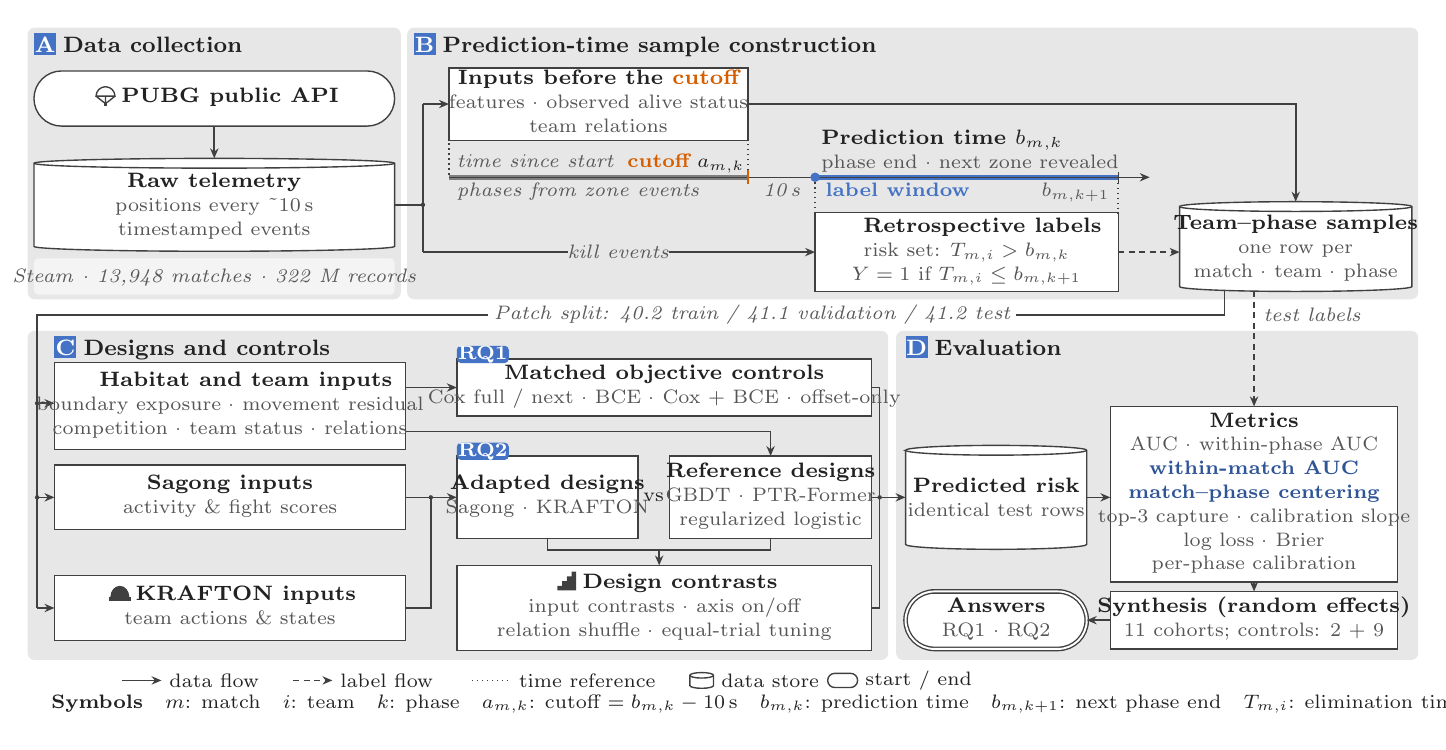
\begin{tikzpicture}
\useasboundingbox (0,-0.21) rectangle ({17.8cm-4pt},8.61);
% ============================ PANELS & STRIPS ============================
% ---- panel A: Data collection
\fill[panel] (0,5.16) rectangle (4.74,8.61);
\fill[blueC] (0.08,8.26) rectangle (0.36,8.54);
% ---- panel B: Prediction-time sample construction
\fill[panel] (4.82,5.16) rectangle (17.659,8.61);
\fill[blueC] (4.9,8.26) rectangle (5.18,8.54);
% ---- panel C: Designs and analyses
\fill[panel] (0,0.58) rectangle (10.929,4.76);
\fill[blueC] (0.34,4.41) rectangle (0.62,4.69);
% ---- panel D: Evaluation
\fill[panel] (11.029,0.58) rectangle (17.659,4.76);
\fill[blueC] (11.149,4.41) rectangle (11.429,4.69);
\fill[stripF,rounded corners=1.5pt] (0.08,5.22) rectangle (4.66,5.68);
% ============================ TOP ZONE BOXES ============================
% A1 (pill)
\draw[box,rounded corners=0.35cm] (0.08,7.36) rectangle (4.66,8.06);
% A2 (cyl)
\cyl{box}{0.08}{5.77}{4.66}{6.95}
% BI: inputs, spans the input window of the time axis (axis start .. cut)
\draw[box] (5.35,7.18) rectangle (9.15,8.1);
% BL: labels, spans the label window of the time axis (prediction time .. next phase end)
\draw[box] (10.0,5.26) rectangle (13.85,6.26);
% B4 (cyl)
\cyl{box}{14.629}{5.26}{17.579}{6.4}
% ============================ BOTTOM ZONE BOXES ============================
% C1 (ours)
\draw[box] (0.34,3.25) rectangle (4.80,4.36);
% C2 (box)
\draw[box] (0.34,2.235) rectangle (4.80,3.055);
% C3 (box)
\draw[box] (0.34,0.83) rectangle (4.80,1.65);
% M1 (ours)
\draw[box] (5.45,3.68) rectangle (10.72,4.40);
% M2A: adapted designs (left of the RQ2 pair)
\draw[box] (5.45,2.12) rectangle (7.75,3.17);
% M2O: our designs (right of the RQ2 pair)
\draw[box] (8.15,2.12) rectangle (10.72,3.17);
% M3 (box)
\draw[box] (5.45,0.70) rectangle (10.72,1.78);
% D1 (cyl)
\cyl{box}{11.149}{1.985}{13.45}{3.305}
% D2 (box)
\draw[box] (13.75,1.57) rectangle (17.40,3.80);
% D3 (box)
\draw[box] (13.75,0.72) rectangle (17.40,1.45);
% END (endpill)
\draw[box,double=white,double distance=0.7pt,rounded corners=0.365cm] (11.149,0.72) rectangle (13.45,1.45);
\fill[blueC,rounded corners=1.5pt] (5.45,4.35) rectangle (6.11,4.57);
\fill[blueC,rounded corners=1.5pt] (5.45,3.12) rectangle (6.11,3.34);
% ============================ TIME AXIS (panel B, between the inputs and the labels) ============================
% windows on the axis: inputs (axis start .. cut, grey) and label window (prediction time .. next phase end, blue)
\fill[greyD] (5.35,6.68) rectangle (9.15,6.74);
\fill[blueC] (10.0,6.68) rectangle (13.85,6.74);
\draw[axis] (5.35,6.71) -- (14.25,6.71);
\draw[verC,line width=0.8pt] (9.15,6.62) -- (9.15,6.8);
\draw[tick] (13.85,6.64) -- (13.85,6.78);
\fill[blueC] (10.0,6.71) circle (0.06);
% time references: each data box spans its window
\draw[tref] (5.35,6.74) -- (5.35,7.18);
\draw[tref] (9.15,6.8) -- (9.15,7.18);
\draw[tref] (10.0,6.65) -- (10.0,6.26);
\draw[tref] (13.85,6.64) -- (13.85,6.26);
% ============================ EDGES ============================
% edge A1A2: A1 -> A2
\draw[edge] (2.37,7.36) -- (2.37,6.95);
% edge RAW: A2 -> junction -> inputs (records before the cut) / labels (kill events)
\draw[lineplain] (4.66,6.36) -- (5.02,6.36);
\draw[lineplain] (5.02,5.76) -- (5.02,7.64);
\fill[ink] (5.02,6.36) circle (0.028);
\draw[edge] (5.02,7.64) -- (5.35,7.64);
\draw[lineplain] (5.02,5.76) -- (6.86,5.76);
\draw[edge] (8.14,5.76) -- (10.0,5.76);
% edge BIB4: inputs -> samples (data flow)
\draw[edge] (9.15,7.64) -- (16.104,7.64) -- (16.104,6.4);
% edge BLB4: labels -> samples (label flow)
\draw[dedge] (13.85,5.76) -- (14.629,5.76);
% edge RET: return line B4 -> down the left margin of C (bus), interrupted by its label "12 cohorts . match-level split 8:1:1"
\draw[lineplain] (15.2,5.275) -- (15.2,4.96) -- (11.17,4.96);
\draw[lineplain] (7.23,4.96) -- (0.12,4.96) -- (0.12,1.24);
% edge RETC1: return bus -> C1
\draw[edge] (0.12,3.84) -- (0.34,3.84);
% edge RETC2: return bus -> C2
\draw[edge] (0.12,2.645) -- (0.34,2.645);
% edge RETC3: return bus -> C3
\draw[edge] (0.12,1.24) -- (0.34,1.24);
\fill[ink] (0.12,3.84) circle (0.028);
\fill[ink] (0.12,2.645) circle (0.028);
% edge DASH: label flow B4 -> D2, straight down ("test labels")
\draw[dedge] (15.575,5.265) -- (15.575,3.80);
% edge C1M1: habitat block -> RQ1 model
\draw[edge] (4.80,4.04) -- (5.45,4.04);
% edge C1M2O: habitat block (+ other team features) -> our designs, below M1, interrupted by its label
\draw[edge] (4.80,3.48) -- (9.435,3.48) -- (9.435,3.17);
% edge C2M2A: Sagong inputs -> adapted designs
\draw[edge] (4.80,2.645) -- (5.45,2.645);
% edge C3M2A: KRAFTON inputs -> joins C2 -> adapted designs
\draw[lineplain] (4.80,1.24) -- (5.12,1.24) -- (5.12,2.645);
\fill[ink] (5.12,2.645) circle (0.028);
% edge M2M3: bracket under the RQ2 pair -> stepwise decomposition
\draw[lineplain] (6.60,2.12) -- (6.60,1.98) -- (9.435,1.98) -- (9.435,2.12);
\draw[edge] (8.02,1.98) -- (8.02,1.78);
% edge M2D1: our designs -> D1 (merged arrowhead)
\draw[edge] (10.72,2.645) -- (11.149,2.645);
% edge M3D1: M3 -> joins M2 -> D1
\draw[lineplain] (10.72,1.24) -- (10.82,1.24) -- (10.82,2.645);
\fill[ink] (10.82,2.645) circle (0.028);
% edge D1D2: D1 -> D2
\draw[edge] (13.45,2.645) -- (13.75,2.645);
% edge D2D3: D2 -> D3
\draw[edge] (15.575,1.57) -- (15.575,1.45);
% edge D3END: D3 -> END
\draw[edge] (13.75,1.085) -- (13.45,1.085);
% edge M1D1: objective controls -> joins the designs' line -> D1
\draw[lineplain] (10.72,4.04) -- (10.82,4.04) -- (10.82,2.645);
% ============================ ZONE SEPARATORS ============================
% ============================ LEGEND ============================
\draw[edge] (1.20,0.32) -- (1.70,0.32);
\draw[dedge] (3.37,0.32) -- (3.87,0.32);
\draw[tref] (5.64,0.32) -- (6.14,0.32);
\cylsmall{box}{8.41}{0.22}{8.71}{0.42}
\draw[box,rounded corners=0.09cm] (10.16,0.23) rectangle (10.54,0.41);
% ============================ TEXT (node t<ID> sits at the centre of box <ID>) ============================
\node[font=\fLetter,anchor=base,align=center,text=white] (taglA) at (0.22,8.298) {A};
\node[font=\fTitle,anchor=base west,align=left] (ttlA) at (0.45,8.298) {Data collection};
\node[font=\fLetter,anchor=base,align=center,text=white] (taglB) at (5.04,8.298) {B};
\node[font=\fTitle,anchor=base west,align=left] (ttlB) at (5.27,8.298) {Prediction-time sample construction};
\node[font=\fLetter,anchor=base,align=center,text=white] (taglC) at (0.48,4.448) {C};
\node[font=\fTitle,anchor=base west,align=left] (ttlC) at (0.71,4.448) {Designs and controls};
\node[font=\fLetter,anchor=base,align=center,text=white] (taglD) at (11.289,4.448) {D};
\node[font=\fTitle,anchor=base west,align=left] (ttlD) at (11.519,4.448) {Evaluation};
\node[font=\fSmallI,anchor=base,align=center,text=greyT] (tstripA) at (2.37,5.375) {Steam\md{}13,948 matches\md{}322 M records};
\node[font=\fBox,align=center] (tA1) at (2.37,7.71) {\rule{0pt}{0.205cm}\icoParachute{}\bT{txtC}{PUBG public API}\rule[-0.095cm]{0pt}{0.095cm}};
\node[font=\fBox,align=center] (tA2) at (2.37,6.329) {\rule{0pt}{0.205cm}\bT{txtC}{Raw telemetry}\\\bD{detC}{positions every \textasciitilde10\,s}\\\bD{detC}{timestamped events}\rule[-0.095cm]{0pt}{0.095cm}};
\node[font=\fBox,align=center] (tBI) at (7.25,7.64) {\rule{0pt}{0.205cm}\bT{txtC}{Inputs before the \textcolor{verC}{cutoff}}\\\bD{detC}{features\md{}observed alive status}\\\bD{detC}{team relations}\rule[-0.095cm]{0pt}{0.095cm}};
\node[font=\fBox,align=center] (tBL) at (11.925,5.76) {\rule{0pt}{0.205cm}\icoCrosshairs{}\bT{txtC}{Retrospective labels}\\\bD{detC}{risk set: $T_{m,i}>b_{m,k}$}\\\bD{detC}{$Y=1$ if $T_{m,i}\le b_{m,k+1}$}\rule[-0.095cm]{0pt}{0.095cm}};
\node[font=\fBox,align=center] (tB4) at (16.104,5.8) {\rule{0pt}{0.205cm}\bT{txtC}{Team--phase samples}\\\bD{detC}{one row per}\\\bD{detC}{match\md{}team\md{}phase}\rule[-0.095cm]{0pt}{0.095cm}};
% time-axis labels: instants above the axis, windows and phase source below
\node[font=\fSmallI,anchor=base west,align=left,text=greyT] (tax0) at (5.45,6.83) {time since start};
\node[font=\fSmall,anchor=base east,align=right] (taxcut) at (9.10,6.83) {\textbf{\textcolor{verC}{cutoff}} $a_{m,k}$};
\node[font=\fBox,anchor=south west,align=left] (taxpt) at (10.08,6.77) {\bT{txtC}{Prediction time $b_{m,k}$}\\\bD{detC}{phase end\md{}next zone revealed}};
\node[font=\fSmallI,anchor=base west,align=left,text=greyT] (tax1) at (5.45,6.46) {phases from zone events};
\node[font=\fSmallI,anchor=base,align=center,text=greyT] (taxgap) at (9.575,6.46) {10\,s};
\node[font=\fSmall,anchor=base,align=center] (taxwin) at (11.05,6.46) {\textbf{\textcolor{blueC}{label window}}};
\node[font=\fSmallI,anchor=base east,align=right,text=greyT] (taxnext) at (13.74,6.46) {$b_{m,k+1}$};
\node[font=\fSmallI,align=center,text=greyT] (tkill) at (7.50,5.76) {kill events};
\node[font=\fBox,align=center] (tC1) at (2.57,3.805) {\rule{0pt}{0.205cm}\icoLeaf{}\bT{txtC}{Habitat and team inputs}\\\bD{detC}{boundary exposure\md{}movement residual}\\\bD{detC}{competition\md{}team status\md{}relations}\rule[-0.095cm]{0pt}{0.095cm}};
\node[font=\fBox,align=center] (tC2) at (2.57,2.645) {\rule{0pt}{0.205cm}\bT{txtC}{Sagong inputs}\\\bD{detC}{activity \& fight scores}\rule[-0.095cm]{0pt}{0.095cm}};
\node[font=\fBox,align=center] (tC3) at (2.57,1.24) {\rule{0pt}{0.205cm}\icoHelmet{}\bT{txtC}{KRAFTON inputs}\\\bD{detC}{team actions \& states}\rule[-0.095cm]{0pt}{0.095cm}};
\node[font=\fBox,align=center] (tM1) at (8.085,4.04) {\rule{0pt}{0.205cm}\bT{txtC}{Matched objective controls}\\\bD{detC}{Cox full / next\md{}BCE\md{}Cox + BCE\md{}offset-only}\rule[-0.095cm]{0pt}{0.095cm}};
\node[font=\fBox,align=center] (tM2A) at (6.60,2.645) {\rule{0pt}{0.205cm}\bT{txtC}{Adapted designs}\\\bD{detC}{Sagong\md{}KRAFTON}\rule[-0.095cm]{0pt}{0.095cm}};
\node[font=\fBox,align=center] (tM2O) at (9.435,2.645) {\rule{0pt}{0.205cm}\bT{txtC}{Reference designs}\\\bD{detC}{GBDT\md{}PTR-Former}\\\bD{detC}{regularized logistic}\rule[-0.095cm]{0pt}{0.095cm}};
\node[font=\fSmall,align=center] (tvs) at (7.95,2.645) {vs};
\node[font=\fBox,align=center] (tM3) at (8.085,1.24) {\rule{0pt}{0.205cm}\icoStairs{}\bT{txtC}{Design contrasts}\\\bD{detC}{input contrasts\md{}axis on/off}\\\bD{detC}{relation shuffle\md{}equal-trial tuning}\rule[-0.095cm]{0pt}{0.095cm}};
\node[font=\fBox,align=center] (tD1) at (12.30,2.614) {\rule{0pt}{0.205cm}\bT{txtC}{Predicted risk}\\\bD{detC}{identical test rows}\rule[-0.095cm]{0pt}{0.095cm}};
\node[font=\fBox,align=center] (tD2) at (15.575,2.685) {\rule{0pt}{0.205cm}\bT{txtC}{Metrics}\\\bD{detC}{AUC\md{}within-phase AUC}\\\bD{detC}{{\bfseries\color{oursT}within-match AUC}}\\\bD{detC}{{\bfseries\color{oursT}match--phase centering}}\\\bD{detC}{top-3 capture\md{}calibration slope}\\\bD{detC}{log loss\md{}Brier}\\\bD{detC}{per-phase calibration}\rule[-0.095cm]{0pt}{0.095cm}};
\node[font=\fBox,align=center] (tD3) at (15.575,1.085) {\rule{0pt}{0.205cm}\bT{txtC}{Synthesis (random effects)}\\\bD{detC}{11 cohorts; controls: 2 + 9}\rule[-0.095cm]{0pt}{0.095cm}};
\node[font=\fBox,align=center] (tEND) at (12.30,1.085) {\rule{0pt}{0.205cm}\bT{txtC}{Answers}\\\bD{detC}{RQ1\md{}RQ2}\rule[-0.095cm]{0pt}{0.095cm}};
\node[font=\fRQ,align=center,text=white] (trq1) at (5.78,4.46) {RQ1};
\node[font=\fRQ,align=center,text=white] (trq2) at (5.78,3.23) {RQ2};
\node[font=\fSmallI,align=center,text=greyT,fill=white,inner sep=2pt] (tret) at (9.2,4.96) {Patch split: 40.2 train / 41.1 validation / 41.2 test};
\node[font=\fSmallI,anchor=west,align=left,text=greyT] (tdash) at (15.695,4.96) {test labels};
\node[font=\fSmall,anchor=west,align=left] (tlg0) at (1.80,0.32) {data flow};
\node[font=\fSmall,anchor=west,align=left] (tlg1) at (3.97,0.32) {label flow};
\node[font=\fSmall,anchor=west,align=left] (tlg6) at (6.24,0.32) {time reference};
\node[font=\fSmall,anchor=west,align=left] (tlg4) at (8.81,0.32) {data store};
\node[font=\fSmall,anchor=west,align=left] (tlg5) at (10.64,0.32) {start / end};
\node[font=\fSmall,anchor=north west,align=left] (tsym) at (0.30,0.14) {\textbf{Symbols}\quad $m$: match\quad $i$: team\quad $k$: phase\quad $a_{m,k}$: cutoff $=b_{m,k}-10$\,s\quad $b_{m,k}$: prediction time\quad $b_{m,k+1}$: next phase end\quad $T_{m,i}$: elimination time};
\end{tikzpicture}
\end{document}
